\subsection{Effect of Gravitational waves on objects}
\subsubsection{Plus polarized effect}
When a plus polarized wave passes through the object, since such gravitational wave makes space-time oscillate in X and Y axes only. So the points in space along axis will come close during compression and go far during stretching. Thus the object itself will be compressed and stretched along the axes, perpendicular to the direction of propagation of wave.

\subsubsection{Cross polarized effect}
When a cross polarized wave passes through the object, since such gravitational wave makes space-time oscillate along the line which makes an inclination of 45$\degree$ with X and Y axes (i.e. along the line $x=y$ and $x=-y$). So the points in space along those line will come close during compression and go far during stretching. Thus the object itself will be compressed and stretched along those lines, perpendicular to the direction of propagation of wave.
\\

Thus for every phase difference of $\pi/2$ we get the shape of object to be as follows
when a plus polarized wave passes and a cross polarized wave passes through a spherical object:

\begin{center}
    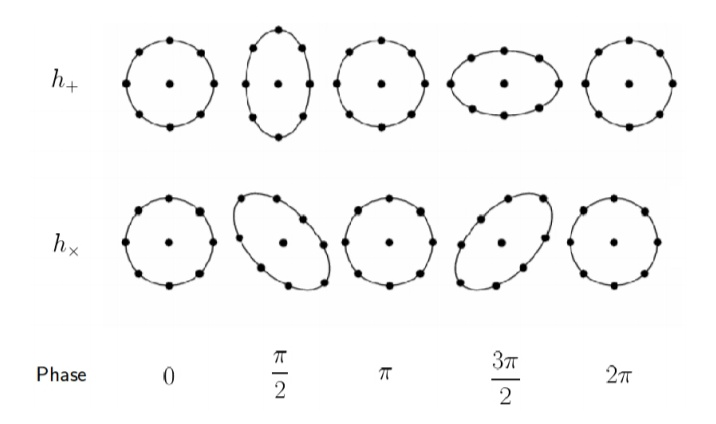
\includegraphics[scale=0.5]{images.tex/effect_of_gw.jpeg}
\end{center}
